% Convolution operator.
% Adapted from https://github.com/PetarV-/TikZ/tree/master/2D%20Convolution

\documentclass[tikz]{standalone}

\usetikzlibrary{matrix, positioning}

\usepackage{xcolor}
\colorlet{myred}{red!80!black}
\colorlet{myblue}{blue!80!black}
\colorlet{mybluee}{myblue!80!black}
\colorlet{mygreen}{green!60!black}
\colorlet{myorange}{orange!70!red!60!black}
\colorlet{mydarkred}{red!30!black}
\colorlet{mydarkblue}{blue!40!black}
\colorlet{mydarkgreen}{green!30!black}

\begin{document}
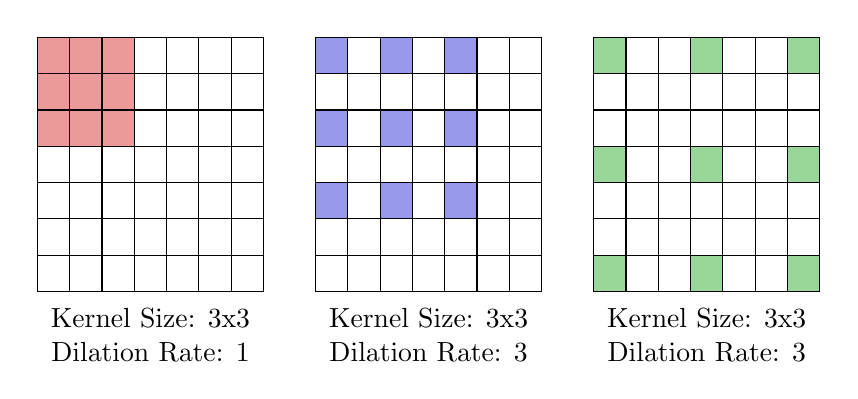
\begin{tikzpicture}[
    2d-arr/.style={matrix of nodes, row sep=-\pgflinewidth, column sep=-\pgflinewidth, nodes={draw}}
  ]

  \matrix (mtr) [2d-arr] {
  |[fill=myred!40]|\phantom{0} & |[fill=myred!40]| \phantom{0} & |[fill=myred!40]| \phantom{0} & \phantom{0} & \phantom{0} & \phantom{0} & \phantom{0}\\
  |[fill=myred!40]|\phantom{0} & |[fill=myred!40]|\phantom{0} & |[fill=myred!40]|\phantom{0} & \phantom{0} & \phantom{0} & \phantom{0} & \phantom{0}\\
  |[fill=myred!40]| \phantom{0} & |[fill=myred!40]| \phantom{0} & 
 |[fill=myred!40]|\phantom{0} & \phantom{0} & \phantom{0} & \phantom{0} & \phantom{0}\\
  \phantom{0} & \phantom{0} & \phantom{0} & \phantom{0} & \phantom{0} & \phantom{0} & \phantom{0}\\
  \phantom{0} & \phantom{0} & \phantom{0} & \phantom{0} & \phantom{0} & \phantom{0} & \phantom{0}\\
  \phantom{0} & \phantom{0} & \phantom{0} & \phantom{0} & \phantom{0} & \phantom{0} & \phantom{0}\\
  \phantom{0} & \phantom{0} & \phantom{0} & \phantom{0} & \phantom{0} & \phantom{0} & \phantom{0}\\
  };

  \node[below=of mtr-5-4] (txt) {Kernel Size: 3x3};
  \node[below=-0.05cm of txt] {Dilation Rate: 1};


  \matrix (mtr2) [2d-arr, right=0.4cm of mtr] {
  |[fill=myblue!40]|\phantom{0} & \phantom{0} & |[fill=myblue!40]| \phantom{0} & \phantom{0} & |[fill=myblue!40]|\phantom{0} & \phantom{0} & \phantom{0}\\
  \phantom{0} & \phantom{0} & \phantom{0} & \phantom{0} & \phantom{0} & \phantom{0} & \phantom{0}\\
  |[fill=myblue!40]| \phantom{0} &  \phantom{0} & 
 |[fill=myblue!40]|\phantom{0} & \phantom{0} & |[fill=myblue!40]|\phantom{0} & \phantom{0} & \phantom{0}\\
  \phantom{0} & \phantom{0} & \phantom{0} & \phantom{0} & \phantom{0} & \phantom{0} & \phantom{0}\\
  |[fill=myblue!40]|\phantom{0} & \phantom{0} & |[fill=myblue!40]|\phantom{0} & \phantom{0} & |[fill=myblue!40]|\phantom{0} & \phantom{0} & \phantom{0}\\
  \phantom{0} & \phantom{0} & \phantom{0} & \phantom{0} & \phantom{0} & \phantom{0} & \phantom{0}\\
  \phantom{0} & \phantom{0} & \phantom{0} & \phantom{0} & \phantom{0} & \phantom{0} & \phantom{0}\\
  };

  \node[below=of mtr2-5-4] (txt) {Kernel Size: 3x3};
  \node[below=-0.05cm of txt] {Dilation Rate: 3};



  \matrix (mtr3) [2d-arr, right=0.4cm of mtr2] {
  |[fill=mygreen!40]|\phantom{0} &  \phantom{0} &  \phantom{0} & |[fill=mygreen!40]|\phantom{0} & \phantom{0} & \phantom{0} & |[fill=mygreen!40]|\phantom{0}\\
  \phantom{0} & \phantom{0} & \phantom{0} & \phantom{0} & \phantom{0} & \phantom{0} & \phantom{0}\\
   \phantom{0} &  \phantom{0} & 
 \phantom{0} & \phantom{0} & \phantom{0} & \phantom{0} & \phantom{0}\\
  |[fill=mygreen!40]|\phantom{0} & \phantom{0} & \phantom{0} & |[fill=mygreen!40]|\phantom{0} & \phantom{0} & \phantom{0} & |[fill=mygreen!40]|\phantom{0}\\
  \phantom{0} & \phantom{0} & \phantom{0} & \phantom{0} & \phantom{0} & \phantom{0} & \phantom{0}\\
  \phantom{0} & \phantom{0} & \phantom{0} & \phantom{0} & \phantom{0} & \phantom{0} & \phantom{0}\\
  |[fill=mygreen!40]|\phantom{0} & \phantom{0} & \phantom{0} & |[fill=mygreen!40]|\phantom{0} & \phantom{0} & \phantom{0} & |[fill=mygreen!40]|\phantom{0}\\
  };

  \node[below=of mtr3-5-4] (txt) {Kernel Size: 3x3};
  \node[below=-0.05cm of txt] {Dilation Rate: 3};

\end{tikzpicture}
\end{document}